\documentclass[12pt, a4paper, ngerman]{article}

% Metadata Setup
\newcommand{\Autor}{Leon Kampwerth}
\newcommand{\Was}{Hausarbeit Digitale Bildverarbeitung}
\newcommand{\Kurs}{TINF20IN}
\newcommand{\MatrikelNummer}{5722356}
\newcommand{\Studiengang}{Digitale Bildverarbeitung}

\title{Perceptually Uniform Color Spaces und der Oklab Farbraum}
\author{\Autor}
\date{22.03.2023}

% SETUP
\usepackage{biblatex} % für bibliografie
\usepackage{hyperref} % für links zum klicken
\usepackage{color}    % für Farben (benötigt für listings)
\usepackage{listings} % code schnipsel
\usepackage[ngerman]{babel} % lokalisierung der Titel (Inhaltsverzeichniss)
\usepackage{bookmark} % bookmarks für das PDF
\usepackage{csquotes} % korrekte quotes
\usepackage[version=3]{acro} % akronyme
\usepackage{geometry} % seitengeometrie (margin etc einstellen)
\usepackage{parskip}  % zeilenabstand bei neuem paragraph statt indentierung
\usepackage{fancyhdr} % header und footer
\usepackage{array}    % für bessere Tabellen
\usepackage{titlesec} % um die Titel anzupassen
\usepackage{plantuml} % PLANTUML_JAR has to be set and --shell-escape
\usepackage{amsfonts} % für \mathbb
\usepackage{placeins} % für \FloatBarrier
\usepackage{nicematrix}
\usepackage{amsmath}
%Für den monsterblock
\usepackage{graphicx}
\usepackage{subcaption}
 
\hypersetup{
  pdfauthor={\Autor},
  pdftitle={\Was},
  hidelinks
}

\geometry{
  a4paper,
  left=25mm,
  right=25mm,
  headheight=125mm,
  top=35mm,
  bottom=30mm,
  footskip=15mm
}

% title setup 
% make paragraph have a newline
\titleformat{\paragraph}
{\normalfont\normalsize\bfseries}{\theparagraph}{1em}{}
\titlespacing*{\paragraph}
{0pt}{3.25ex plus 1ex minus .2ex}{1.5ex plus .2ex}

% add bibliography
\addbibresource{bibliography.bib}

% header and footer setup
\pagestyle{fancy}
\fancyhf{}
\rhead{\Was}
\lhead{\leftmark}
\lfoot{Autor: \Autor, Kurs: \Kurs}
\rfoot{Seite \thepage}
\renewcommand{\headrulewidth}{1pt}
\renewcommand{\footrulewidth}{1pt}
\fancypagestyle{simple}{
  \fancyhf{}
  \rhead{\Was}
  \lfoot{Autor: \Autor, Kurs: \Kurs}
  \rfoot{Seite \thepage}
}

% acronyms
\acsetup{
  list/display = used,
  pages/display = first
}

%Offizele Akronyme

\newcommand{\reals}{\ensuremath{\mathbb{R}}}
\newcommand{\natnums}{\ensuremath{\mathbb{N}}}

% code snippet setup
\renewcommand{\lstlistingname}{Code-Auszug}
\renewcommand{\lstlistlistingname}{Liste der Code-Auszüge}

\definecolor{black}{rgb}{0,0,0}
\definecolor{green}{rgb}{0,0.5,0}
\definecolor{orange}{rgb}{1,0.45,0.13}		
\definecolor{brown}{rgb}{0.69,0.31,0.31}

% python
\lstdefinelanguage{Python}{
  morekeywords={import, def, from, for, in, if, else, return, True, False, catch, return, null, switch, if, in, while, do, else, case, break},
  morecomment=[l]\#,
  morestring=[b]",
  morestring=[b]""",
  morestring=[b]'
}

\lstdefinestyle{light}{
  % General design
  basicstyle={\footnotesize\ttfamily},   
  frame=b,
  % line-numbers
  xleftmargin={0.75cm},
  numbers=left,
  stepnumber=1,
  firstnumber=1,
  numberfirstline=true,	
  % Quellcode design
  identifierstyle=\color{black},
  keywordstyle=\color{blue}\bfseries,
  ndkeywordstyle=\color{green}\bfseries,
  stringstyle=\color{orange}\ttfamily,
  commentstyle=\color{brown}\ttfamily,
  % Quellcode
  alsodigit={.:;},
  tabsize=2,
  showtabs=false,
  showspaces=false,
  showstringspaces=false,
  extendedchars=true,
  breaklines=true,
}

\begin{document}
\raggedright % sorgt dafür das alles strikt links ausgerichtet wird (und sorgt für mehr seiten)


% Titlepage
\makeatletter
\begin{titlepage}
  \begin{center}
    \vspace*{1cm}
    {\Huge\scshape \Was}\\[2cm]
    \begin{center}
      \linespread{1}\Huge \@title\\[2cm]
    \end{center}
    {\large \Studiengang}\\
    {\large Duale Hochschule Baden-Württemberg\\ Stuttgart}\\[2cm]
    {\large von}\\
    {\large\bfseries \@author}
    \vfill
  \end{center}
  \begin{tabular}{l@{\hspace{2cm}}l}
    Matrikelnummer: & \MatrikelNummer \\
    Abgabedatum:    & \@date          \\
  \end{tabular}
\end{titlepage}
\makeatother

% Table of content
\tableofcontents
\newpage

\thispagestyle{simple}
\printacronyms[name=Abkürzungsverzeichnis, heading=section*]
\newpage

%%%%%%
% Content here
%%%%%% 

\section{Farben und Farbräume}
Was ist Farbe? Das ist eine Frage die sehr einfach zu Beantworten scheint, da fast jeder Farben sehen kann. 
Die Encyclopedia Britannica definiert Farbe sinngemäß als Eigenschaft eines Objektes, die durch dessen Farbton, 
Helligkeit und Sättigung beschrieben werden kann. In der Physik werden Farben mit Elektromagnetischer Strahlung in einem
bestimmten Bereich des elektromagnetischen Spektrums beschrieben, der für das menschliche Auge sichtbar ist~\cite{Nassau_2023}.
Gerade hier liegt ein Problem vor, da Farben sowohl Phasikalisch erklärt werden können, 
aber auch Teil der Menschlichen wahrnehmeung sind.

\paragraph{Farbwahrnehmung durch das menschliche Auge}
Die Farbwahrnehmung des Menschen besteht aus mehreren Schritten, 
welche von dem Einfallen der Lichtstrahlen in das Auge bis zur Interpretation der Farbe durch das Gehirn reichen.
Im Auge fällt das Licht auf die Netzhaut, wo sich Zapfen- und Stäbchenzellen befinden, 
welche Photorezeptoren sind, die das Licht in Signale für das Hirn umwandeln.
Für die Farbwahrnehmung sind die Zapfen zuständig, von denen es drei Arten gibt, welche auf unterschieliche Wellenlängen reagieren.
S-Zapfen reagieren auf Wellenlängen im blauen Bereich des sichtbaren Spetrums (ca. 420nm), 
M-Zapfen auf Wellenlängen im grünen Bereich (ca. 530nm) und L-Zapfen auf Wellenlängen im gelb-grünen Bereich (ca. 560nm).
Auch wenn der L-Zapfen auf Licht im gelb-grünen Bereich am stärksten reagiert, 
ist er am wichtigsten für die Wahrnehmung von Rot und wird daher auch als Rotrezeptor bezeichnet~\cite{Zapfen_Auge_2023}.
Die Farbwahrnehmung des Menschen entsteht durch das zusammenspiel der drei Zapfen, 
die, wie in Grafik~\ref{fig:LMS} zu erkennen, durch die Wellenlängen unterschiedlich stark angeregt werden. 
Dies kann auch dafür sorgen, dass unterschiedliche Lichtspektren als dieselbe Farbe wahrgenommen werden, 
da sie die unterschiedlichen Zapfen in gleicher Weise erregen. 
So ist es möglich, dass Displays nur durch die Kombination der drei Grundfarben Rot, Grün und Blau 
so viele Farben darstellen können ~\cite{Ottosson_2020}.

\begin{figure}
  \centering
  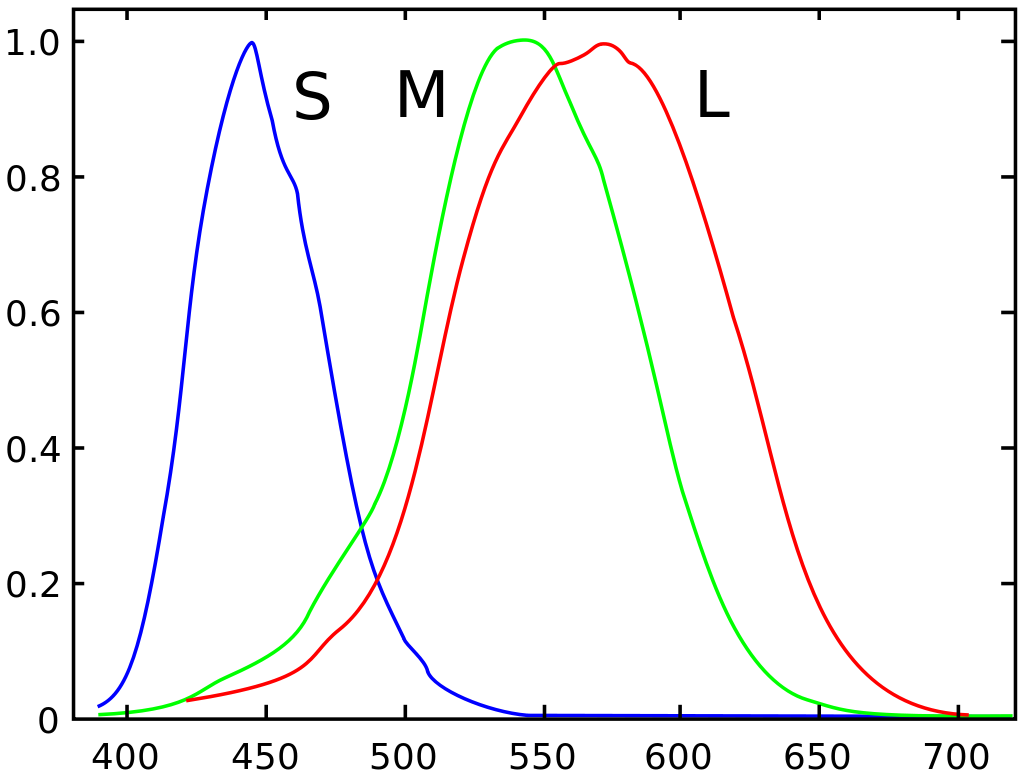
\includegraphics[width=0.5\textwidth]{Grafiken/LMS.png}
  \caption{Normalisierte Empfindlichkeitsspektren menschlicher Zapfenzellen. X Achse: Wellenlänge in nm, Y Achse: Empfindlichkeit, anteilig. Quelle: \cite{LMS_color_space_2023}}
  \label{fig:LMS}
\end{figure}

\paragraph{Farbinterpretation durch das Gehirn}
Die Signale der Zapfen werden im Hirn verarbeitet und interpretiert. 
Dabei werden die Farben durch den Mensch in Form unterschiedlicher Farbeigenschaften wahrgenommen, 
die nicht als physikalische Eigenschaften der Farbe definiert werden können~\cite{Ottosson_2020}.
Zu diesen Farbeigenschaften zählen der Farbton, die Leuchtkraft, die Helligkeit, das Chroma und die Sättigung.
Wichtig ist hier, dass die Wahrnehmung dieser Eigenschaften durch viele psychologische Phenomene beeinflusst wird.
Die chromatische Anpassung beschreibt zum Beispiel die Fähigkeit der menschlichen Farbwahrnehmung, 
bei der Betrachtung eines reflektierenden Objekts vom Weißpunkt der beleuchtenden Lichtquelle zu abstrahieren. 
Für das menschliche Auge sieht ein weißes Blatt Papier weiß aus, egal ob die Beleuchtung bläulich oder gelblich ist.
Weitere solcher effekte sind der Bezold-Brücke Effekt und der Abney Effekt, welche sich auf die wahrnehmeung des Farbtons auswirken,
der Stevens Effekt, welcher sich auf den Kontrast auswirkt und der Helmholtz-Kohlrausch Effekt, der sich auf die Leuchtkraft auswirkt.
All diese Effekte sorgen dafür das die Farbwahrnehmung des Menschen schwer zu beschreiben ist und Modelle, die dies Versuchen sehr komplex werden können~\cite{Color_appearance_model_2023}.

\subsection{Farbräume}
Ein Farbsystem stellt das Grundprinzip einer Farbmischung dar, 
beispielsweise durch das Mischen der Lichtfarben Rot, Grün und Blau oder durch das Mischen von Farbpigmenten.
Farbmodelle werden aus einem solchen Farbsystem abgeleitet und ordnen Farben einen eindeutigen Wert (Farborte) zu.
Farbmodelle sind häufig dreidimensional, damit sie einfach visualisiert werden können.
Ein Farbraum wiederum beschreibt alle Farben eines Farbmodells, die durch farbgebende Methoden tatsächlich ausgegeben werden können~\cite{Farbraum_2023}.
Ein Beispiel ist der sRGB Farbraum, welcher ursprünglich für CRTs entwickelt wurde, aber auch heute noch von vielen Displays verwendet wird~\cite{sRGB-Farbraum_2019}.
Die darstellbaren Farben bilden innerhalb des Farbmodells einen Körper, der als Gamut bezeichnet wird.

\subsection{Farbeigenschaften} 
Abgesehen von den von RGB bekannten Farbdimensionen, welche den Anteil der Grundfarben Rot, Grün und Blau beschreiben, 
gibt es noch weitere mögliche Farbdimensionen. Diese Dimensionen nehmen Bezug auf die Farbeigenschaften, nach denen die Farben beschrieben werden können.
Diese Farbeigenschaften stehen im Bezug zueinander und beeinflussen sich teilweise gegenseitig~\ref{fig:ExColordimension}.

\paragraph{Farbton}
Der Farbton (eng. hue) ist eine Eigenschaft der visuellen Wahrnehmung, in welcher eine Fläche 
ähnlich zu einer der Farben rot, gelb, grün oder blau erscheint oder eine Kombination von 
aneinanderliegenden Paaren dieser Farben in einem geschlossenen Farbring ähnelt (vgl. Grafik \ref{fig:Hue})~\cite{Darktable_2023}. 

\begin{figure}
  \centering
  
\includegraphics[width=0.5\textwidth]{Grafiken/Farbring.png}
  \caption{Beispiel eines Farbrings. Quelle: \cite{Hue_2023}}
  \label{fig:Hue}
\end{figure}

\paragraph{Leuchtkraft (und Brillanz)}
Leuchtkraft (eng. brightness) ist eine Eigenschaft der visuellen Wahrnehmung, 
nach der eine Fläche mehr oder weniger Licht zu emmitieren oder zu reflektieren scheint. 
Die Brillanz (eng. brilliance) ist die Leuchtkraft einer Fläche relativ betrachtet zu ihrer Umgebung.
Leuchtkraft ist ein absoluter Wert, während Brillanz in Relation zur Umgebung steht.
Da bei der Bildverarbeitung eine Erhöhung der Leuchtkraft auch die Brillanz erhöht, 
werden diese Begriffe häufig synonym verwendet~\cite{Darktable_2023}.

\paragraph{Helligkeit}
Die Helligkeit (eng. lightness) einer Fläche beschreibt die Leuchtkraft der Fläche 
relativ zu einer ähnlich beleuteten weißen oder stark reflektierenden Fläche~\cite{Darktable_2023}.

\paragraph{Chroma (Buntheit)}
Chroma beschreibt die Farbigkeit einer Fläche, beurteilt im verhältnis zur Leuchtkraft 
einer ähnlich beleuchteten grauen oder weißen Fläche~\cite{Darktable_2023}. 

\paragraph{Sättigung}
Die Sättigung (eng. saturation) ist die Farbigkeit einer Fläche im verhältnis zu ihrer Leuchtkraft~\cite{Darktable_2023}.

\begin{figure}
  \centering
  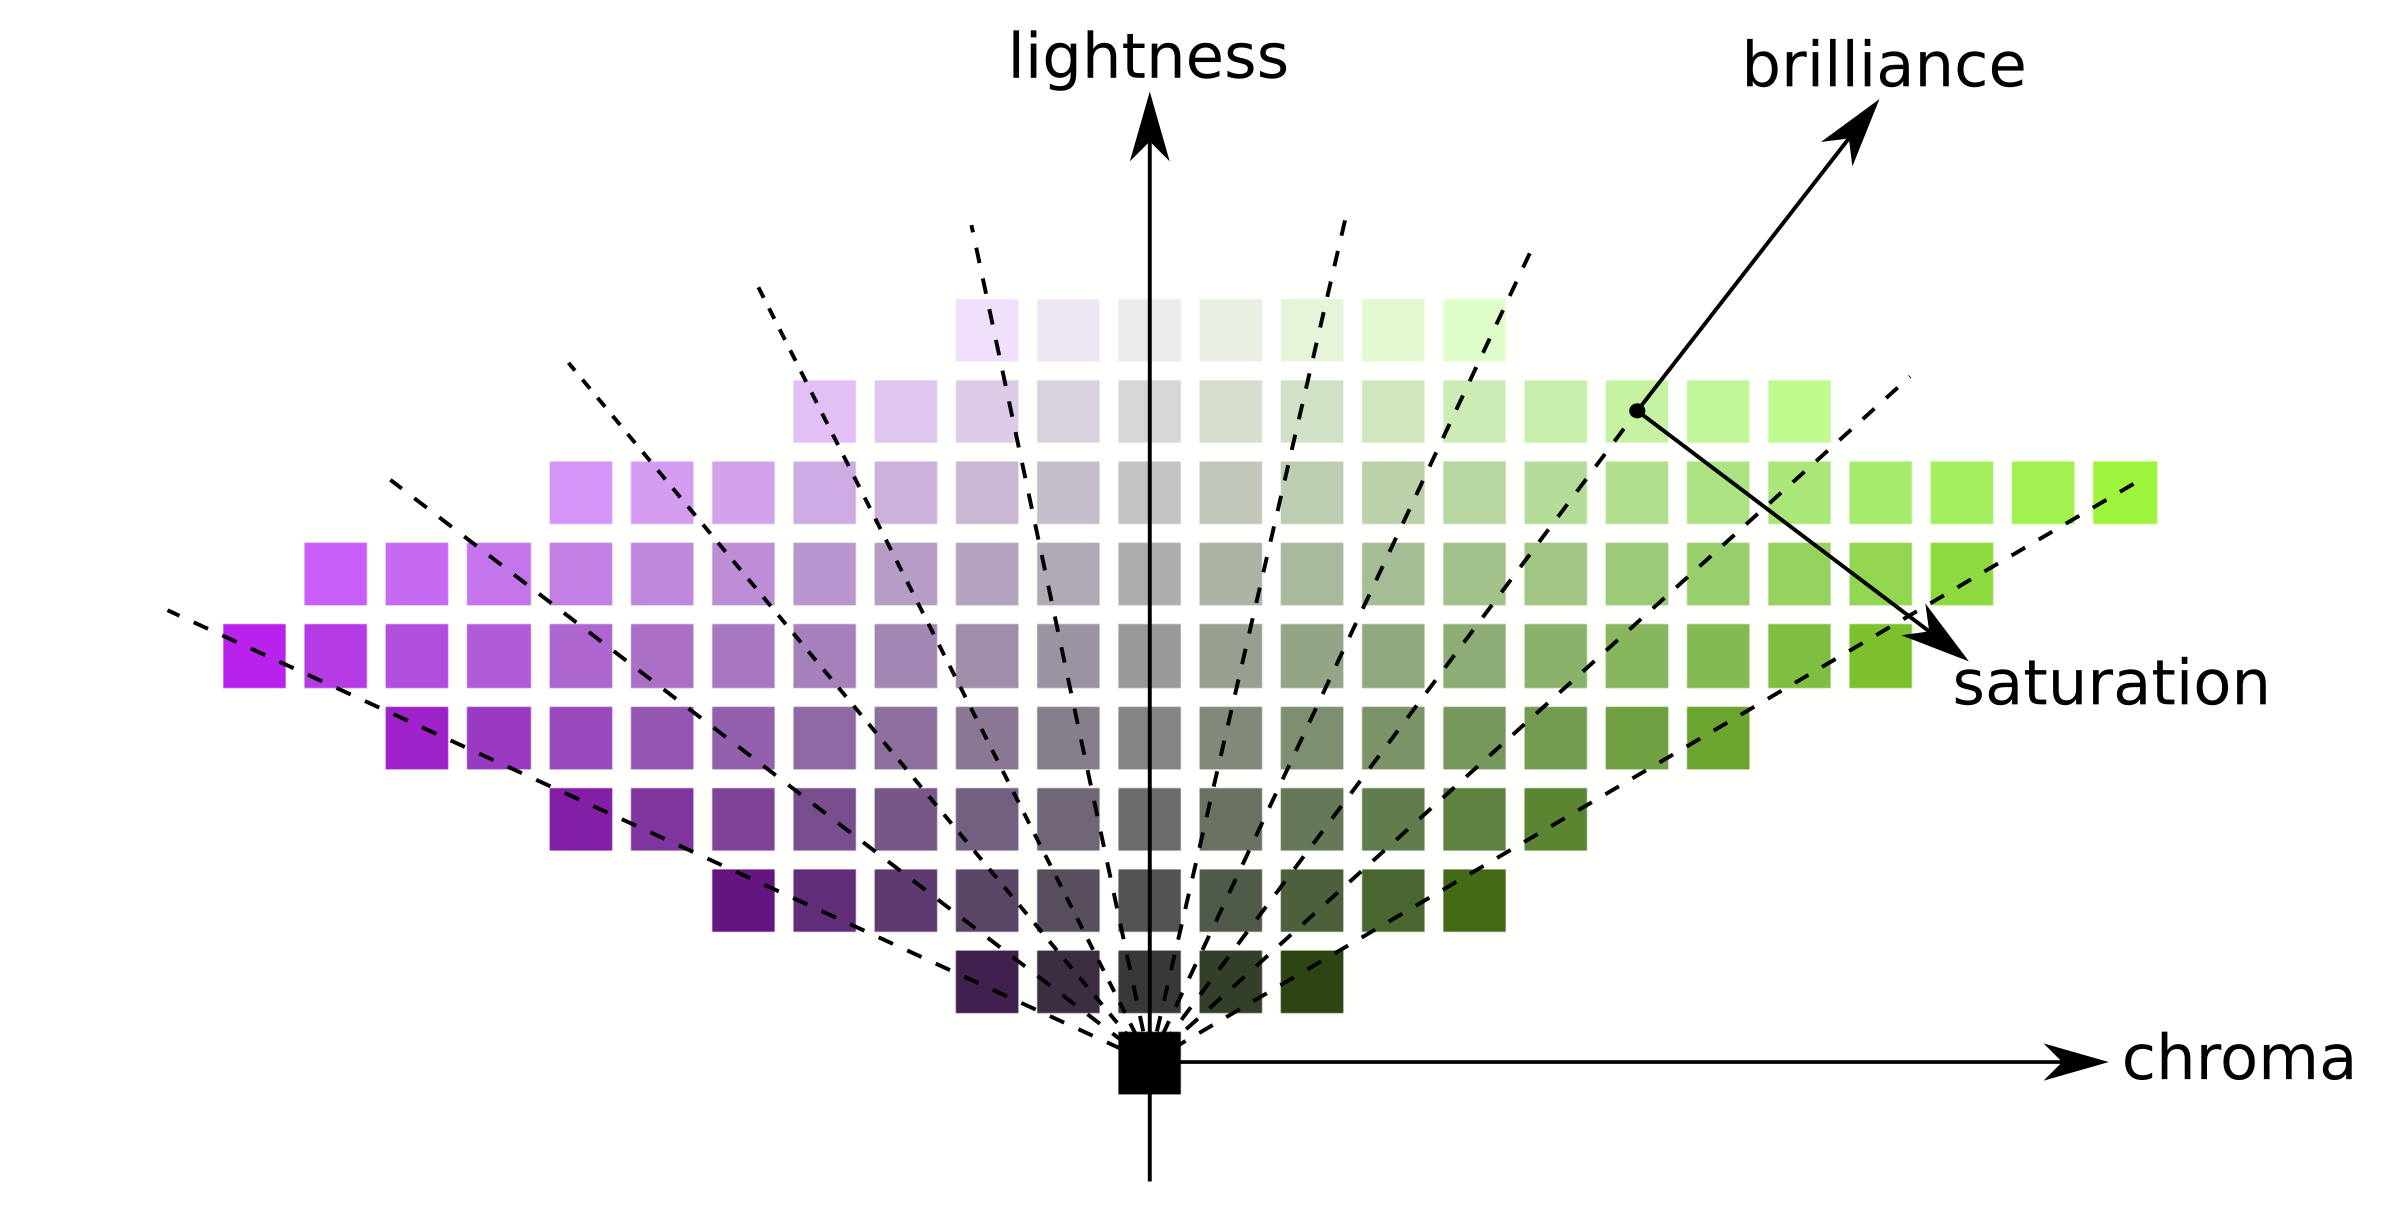
\includegraphics[width=\textwidth]{Grafiken/KoordinatenFarbeigenschaften.png}
  \caption{Beispiel für den Zusammenhang zwischen den Farbeigenschaften. Quelle: \cite{Darktable_2023}}
  \label{fig:ExColordimension}
\end{figure}

\subsection{Unterschieliche Farbräume}
Farben können in vielen unterschiedlichen Farbräumen dargestellt werden. 
Dabei braucht jede Farbe unabhängig vom Farbraum mindestens drei Werte, um beschrieben werden zu können.
Zum einen eine Metrik für Helligkeit oder Leuchtkraft und zum anderen zwei Metriken für die Chromazität 
(nicht zu verwechseln mit Chroma). 
Diese zwei Metriken können zum Beispiel Farbton und Buntheit/Chroma oder komplementäre Farbkoordinaten sein~\cite{Darktable_2023}.
Im Folgenden werden einige Farbräume kurz vorgestellt. Diese Farbräume werden im weiteren Verlauf des Artikels nochmal aufgegriffen.

\paragraph{HSV und HSL}
HSV steht für Hue, Saturation und Value und HSL für Hue, Saturation und Lightness.
Beide Farbräume sind alternative Darstellungen des RGB Farbraums. 
HSL und HSV können beide zylindrische Farbkörper (Abbildung \ref{fig:HSV_HSL}) dargestellt werden, 
wobei hue den Winkel und Saturation den Radius definieren.
Die Höhe des Zylinders ist der Wert, der die Helligkeit als Lightness oder Value beschreibt.
HSV oder HSL werden in Endnutzeranwendungen häufig für Color Picker verwendet ~\cite{HSL_and_HSV_2023}.

\begin{figure}
  \centering
  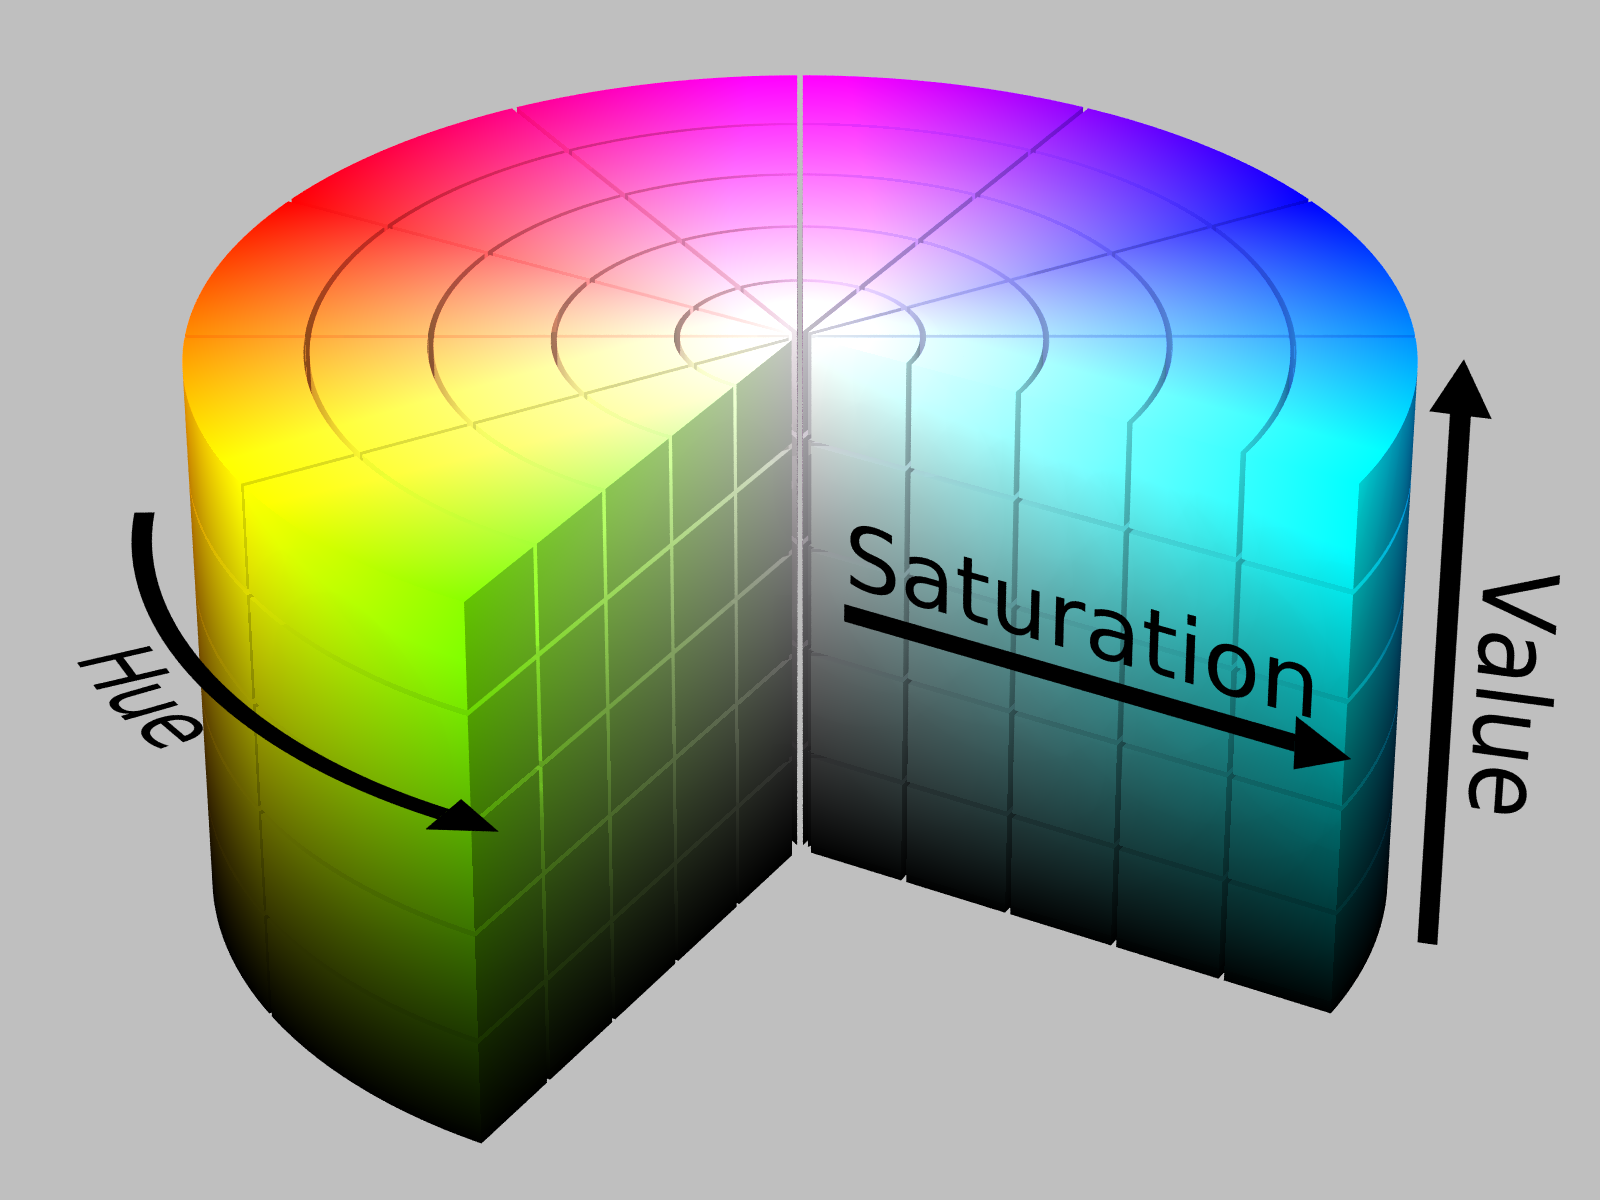
\includegraphics[width=0.48\textwidth]{Grafiken/HSV_Zylinder.png}
  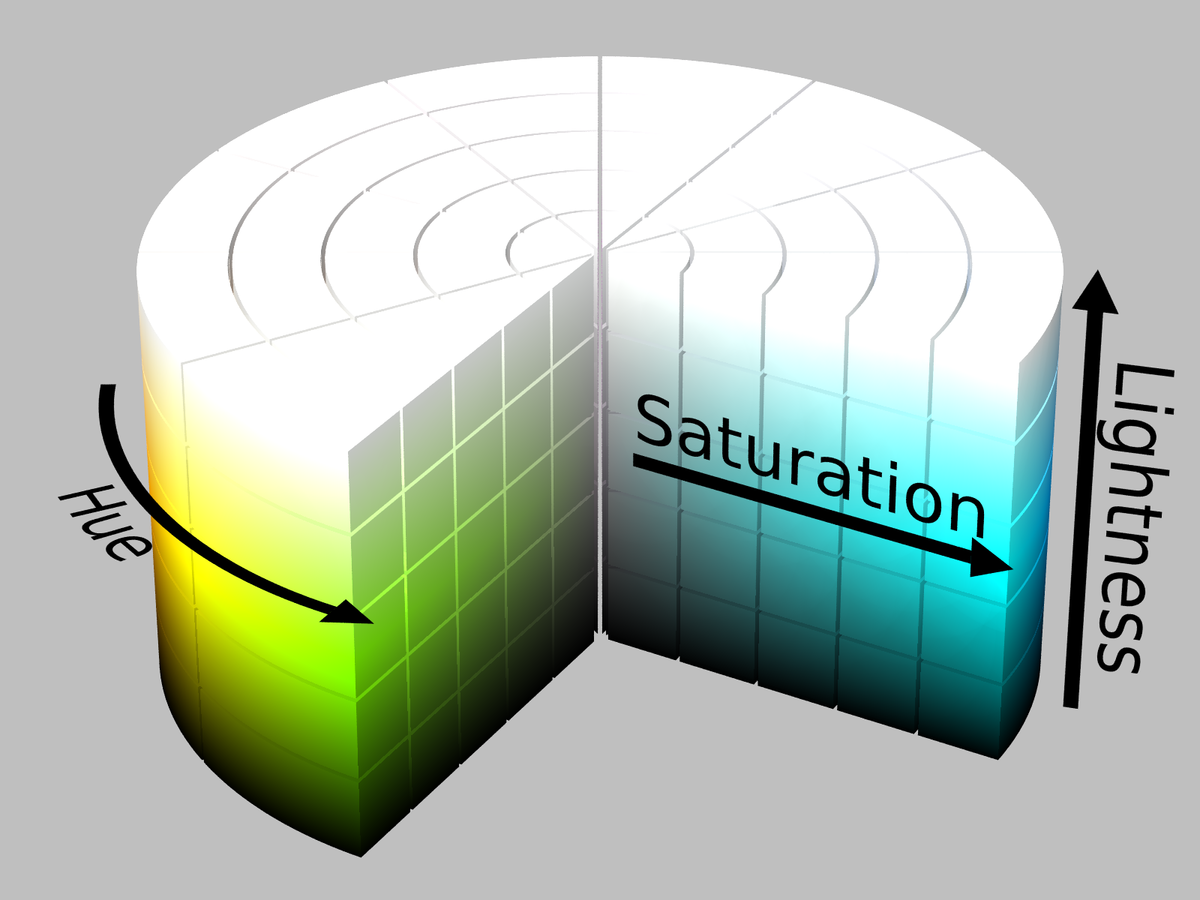
\includegraphics[width=0.48\textwidth]{Grafiken/HSL_Zylinder.png}
  \caption{Beispiel von Farbkörpern für HSV links und HSL rechts. Quelle: ~\cite{HSL_and_HSV_2023}}
  \label{fig:HSV_HSL}
\end{figure}

\paragraph{CIE 1931 XYZ}
Die CIE-Farbräume von 1931 sind die ersten definierten quantitativen Verbindungen zwischen den Verteilungen 
der Wellenlängen im elektromagnetischen sichtbaren Spektrum und den physiologisch wahrgenommenen Farben im menschlichen Farbsehen. 
Bei CIE XYZ werden die drei Farbkoordinaten X, Y und Z verwendet, um die Farbe zu beschreiben.
Dabei ist Y die Lumineszenz, Z ist ähnlich zu Blau im RGB Farbraum und X ist eine Mischung der drei CIE RGB Kurven.
Vorteil ist hier, dass bei einem konstanten Y Wert die XZ Fläche alle Farben dieser Lumineszenz enthält~\cite{CIE_1931_color_space_2023}.

\paragraph{CIELAB}
Der CIELAB Farbraum wurde 1976 von der CIE entwickelt.
CIELAB hat drei dinemsionen und erstreckt sich über den gesamten Gamut des menschlichen Farbsehens (siehe Grafik \ref{fig:CIELAB}).
Die drei Farbkoordinaten orientieren sich ebenfalls an der menschlichen Wahrnehmung, 
wo Rot und Grün, Blau und Gelb, sowie Schwarz und Weiß als Gegenfarben wahrgenommen werden.
Dies bedeutet, dass die Farben sich ausschließen und es zum Beispiel kein rötliches Grün gibt ~\cite{Becker-Carus_Wendt_2017}.
Um dies aufzugreifen werden die Farbkoordinaten L, a und b verwendet.
Die L-Achse ist die Helligkeit und definiert 0 als Schwarz und 100 als Weiß.
Die a-Achse ist eine Relative Achse für die Farbtonkomplementarität von Rot und Grün.
Negative Werte gehen in Richtung Grün, positive Werte in Richtung Rot.
Die b-Achse ist eine Relative Achse für die Farbtonkomplementarität von Blau und Gelb.
Negative Werte gehen in Richtung Blau, positive Werte in Richtung Gelb.
CIELAB wird immer in relation zu einem Referenzweiß definiert, 
wofür CIE die Nutzung von CIE Standard illuminant D65 empfiehlt ~\cite{CIELAB_color_space_2023}.

\begin{figure}
  \centering
  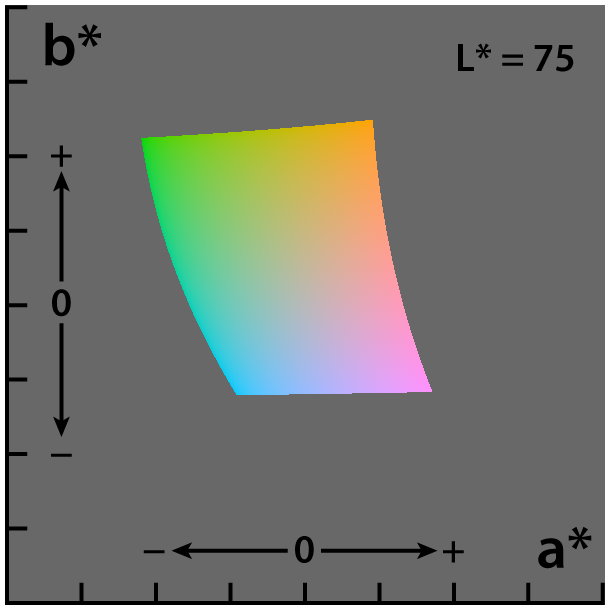
\includegraphics[width=0.29\textwidth]{Grafiken/CIELAB1.png}
  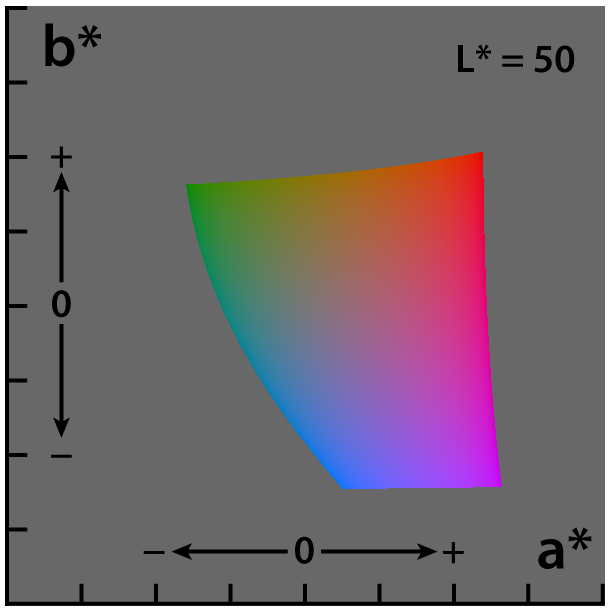
\includegraphics[width=0.29\textwidth]{Grafiken/CIELAB2.png}
  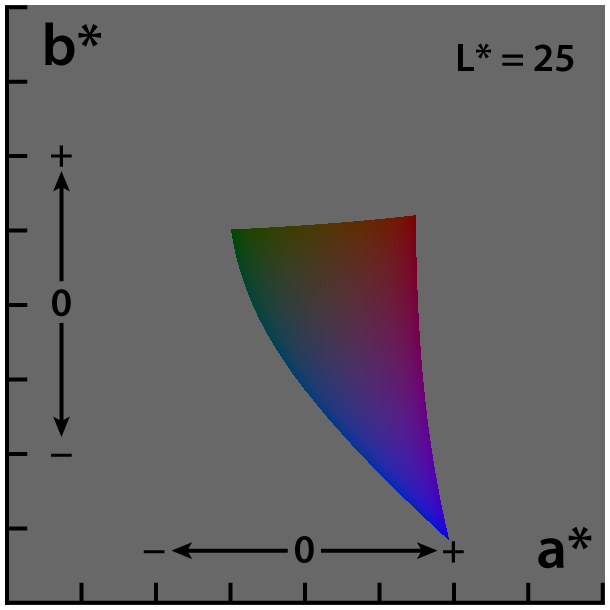
\includegraphics[width=0.29\textwidth]{Grafiken/CIELAB3.png}
  \caption{a*b* Farbebene des CIELAB Farbraumes bei unterschiedlichen L* Werten. Quelle: ~\cite{CIELAB_color_space_2023}}
  \label{fig:CIELAB}
\end{figure}

\paragraph{CAM16-UCS}
In der Farbmetrik ist der OSA-UCS (Optical Society of America Uniform Color Space) ein Farbraum, 
der erstmals 1947 veröffentlicht und vom Committee on Uniform Color Scales der Optical Society of America entwickelt wurde.
Der Ausschuss beschloss, dass eine neue Form verwendet werden muss, 
um einheitliche Farbunterschiede in jeder Richtung genau darstellen zu können.
Die drei dimensionen des Farbraumes sind sehr ähnlich zu CIELAB.
Die L-Achse ist die Helligkeit, die j-Achse ist die Farbtonkomplementarität von Blau und Gelb, 
wobei positive Werte gelber sind und negative Werte blauer sind.
Die g-Achse ist die Farbtonkomplementarität von Rot und Grün, 
wobei positive Werte grüner sind und negative Werte sind pinker ~\cite{OSA-UCS_2023}.

\paragraph{IPT}
Der IPT Farbraum ist ein dreidimensionaler Farbraum.
I steht für die Intensität und P und T ähneln a* und b* von CLAB. 
P beschreibt die Rot-Grün Dimension und T beschreibt die Blau-Gelb Dimension.
Die Vorteile von IPT sind, dass es eine bessere Repräsentation von hue 
in Anlehnung an die menschliche Wahrnehmung bietet. 
Außerdem ist IPT sehr simpel Konzipiert und lässt sich sehr einfach aus dem CIEXYZ Farbraum berechnen ~\cite{Ebner_1998}.

\section{Der Oklab Farbraum}
Das korrekte Darstellen von Farben durch Software ist heutzutage kein Problem mehr, 
anders sieht es bei der der Manipulation von Farben aus.
Typische Farboperationen in Software sind unter anderem das realistische rendern von Bildern, 
das stilisieren und bearbeiten von Bildern, digitales Malen und das Erstellen von Farbverläufen. 
Um dies zu ermöglichen können drei unterschiedliche Vorgehensweisen verwendet werden ~\cite{Ottosson_2020}.
\begin{itemize}
  \item \textbf{Nacharmen des Verhaltens von echtem Licht und Materialien.} Beispielsweise das hinzufügen von Lens Blur, das Hinzufügen von realistischem Nebel oder Raytracing.
  \item \textbf{Nacharmen der menschlichen Farbwahrnehmung,} mit dem Ziel eine intuitive und nachvollziehbare Farbmanipulation zu ermöglichen. Zum Beispiel für das Anpassen des Chroma ohne die Farbe oder Helligkeit zu verändern, das erstellen einheitlich aussehender Farbverläufe oder das monocromatisieren von Bildern ohne deren empfundene Helligkeit zu verändern ~\cite{Oklab_2020}.
  \item \textbf{Stilisierte Operationen ohne Realitätsbezug.} 
\end{itemize}

\subsection{Farbverarbeitung heute}
Da Farbe sowohl eine physikalische als auch psychologische Komponente hat, könnte man nun denken, 
dass Farbverarbeitung in Farbräumen auf Basis der physikalischen Interaktion in der echten Welt oder 
auf Basis der menschlichen Wahrnehmeung erfolgen sollte.
Beides ist aber meistens nicht der Fall, da die meisten Programme der einfachheit halber den weit verbreiteten sRGB Farbraumsystem verwenden.
Auch Bildbearbeitungsprogramme wie Photoshop nutzen meistens einfach denselben Farbraum, 
in dem die Bilder gespeichert werden, um Manipulationen durchzuführen. 
Zum einen werden so meist Farbräume verwendet, die für die Farbreproduktion entwickelt wurden, 
statt welche für das durchführen von Berechnungen.
Zum anderen werden immer die Farbräume verwendet, in denen das Bild gespeichert ist, 
was zu inkonsistenten Ergebnissen zwischen verschiedenen Bildformaten führen kann.
Dies sorgt dafür, dass Farbverarbeitung zu einem nebenprodukt der Defonition des Farbraums wird und 
mit sRGB als verbreiteter Standard ist die definiert danach, wie CRT displays in den 80ern Funktioniert haben.
Um dieses Problem zu beheben wurden über die Jahre viele Funktionen in den Bildbearbeitungsprogrammen implementiert, 
diese sollten das Verhalten an die menschliche Wahrnehmung oder das physikalische Verhalten von Licht anpassen. 
Dennoch wurde der zugrundeliegende Fehler eines nicht zweckdienlichen Farbraumsystems nicht behoben ~\cite{Ottosson_2020}.

Um die Probleme mit der Bildbearbeitung in nicht geeigneten Farbräumen zu visualisieren folgen nun ein paar Beispiele. 
In diesen Beispielen wird der gleiche Farbverlauf mit der drei unterschiedlichen Farbräumen erzeugt, 
der erste basiert auf einem Farbraum der an die menschliche Wahrnehmung angepasst ist, 
der zweite ist ein linearer Farbraum und veranschaulicht gut die physikalische Mischung von Licht, 
der dritte ist ein Farbverlauf in sRGB.
Hier können nun einige unterschiede zwischen den Farbräumen beobachtet werden.
\begin{itemize}
  \item Weder sRGB noch der lineare Farbraum sind in der Lage Farben mit Weiß zu mischen, ohne dass der eindruck eines konstanten Hue aufrechterhalten wird. Besonders gut erkennbar ist dies bei dem blauen Farbverlauf in Grafik \ref{fig:vergleich_white}.
  \item sRGB dunkelt Farben stark ab, wenn unterschiedliche Farben mit hoher Sättigung gemischt werden. Dies ist besonders gut bei dem Farbverlauf von Grün zu Magenta in Grafik \ref{fig:vergleich_zweifarbig} zu erkennen.
  \item Sowohl sRGB als auch der wahrnehmungsbasierte Farbraum mischen Schwarz und Weiß sehr ähnlich (siehe Grafik \ref{fig:vergleich_white}), während der lineare Farbraum viel heller erscheint. Dies ist der Grund weshalb sRGB manchmal auch als wahrnehmungsbasierter Farbraum bezeichnet wird, trotz all seiner Probleme.
\end{itemize}
In dem Vergleich ist zu erkennen des sRGB weder die menschliche Farbwahrnehmung 
noch das physikalische Verhalten von Licht korrekt abbildet.
Daher ist sRGB nicht für die Farbmanipulation von Bildern geeignet ~\cite{Ottosson_2020}.

\begin{figure}
  \centering
  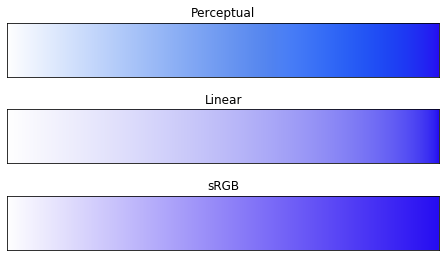
\includegraphics[width=0.29\textwidth]{Grafiken/Farbverlauf/whiteblue.png}
  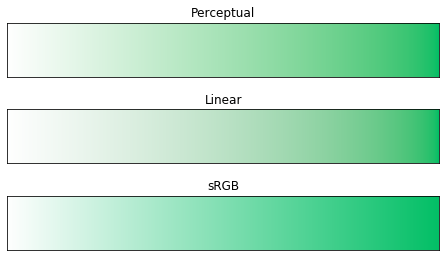
\includegraphics[width=0.29\textwidth]{Grafiken/Farbverlauf/whitegreen.png}
  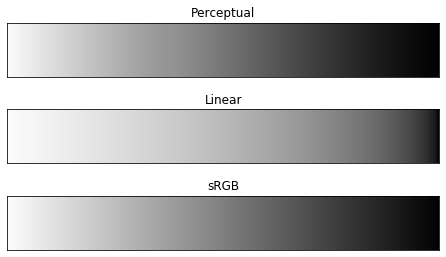
\includegraphics[width=0.29\textwidth]{Grafiken/Farbverlauf/whiteblack.png}
  \caption{Drei Farbverläufe von Weiß zu Blau, Grün und Schwarz. Quelle: ~\cite{Ottosson_2020}}
  \label{fig:vergleich_white}
\end{figure}

\begin{figure}
  \centering
  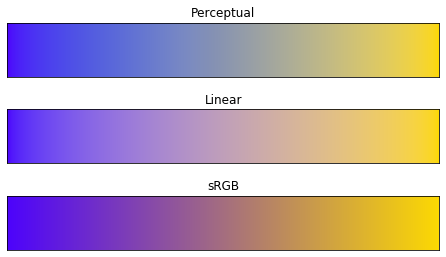
\includegraphics[width=0.29\textwidth]{Grafiken/Farbverlauf/blueyellow.png}
  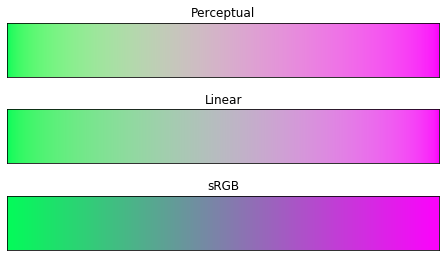
\includegraphics[width=0.29\textwidth]{Grafiken/Farbverlauf/greenmagenta.png}
  \caption{Zwei Farbverläufe, links von Blau nach Gelb, rechts von Grün nach Magenta. Quelle: ~\cite{Ottosson_2020}}
  \label{fig:vergleich_zweifarbig}
\end{figure}

\subsection{Was ist Oklab?}

\paragraph{Motivation für Oklab}
Da nun klar ist, dass die häufig verwendeten Farbräume nicht für die Farbmanipulation geeignet sind, 
muss ein neuer Farbraum entwickelt werden, der diese Aufgabe erfüllt.
Es gibt bereits einige Farbräume, die sich auf die Wahrnehmung von Farben konzentrieren, 
aber alle haben signifikante Nachteile bei der Nutzung für die Bildbearbeitung.
Oklab ist ein neuer wahrnehmungsbasierter Farbraum, der 2020 von Björn Ottosson entwickelt wurde und 
dessen Ziel es ist einfach zu nutzen zu sein und dennoch eine gute Verhersage, 
der  Wahrnehmung von Helligkeit, Chroma und Farbton zu liefern ~\cite{Oklab_2020}.
Der Name \glqq Oklab Color Space\grqq~ steht für \emph{OK Lab Color Space} und meint, 
dass der Farbraum Ok also gut genug ist und es sich dabei um einen Lab Farbraum handelt.

\paragraph{Ziele von Oklab}
Oklab soll ein wahrnehmungsbasierter Farbraum sein, der sich gut für die Bildbearbeitung eignet.
Björn Ottosson hat auf Basis seiner Erfarungen folgende Ziele für Oklab definiert ~\cite{Oklab_2020}:
\begin{enumerate}
  \item Der Farbraum soll wie CIELAB auf der Gegenfarbentheorie basieren.
  \item Der Farbraum soll Helligkeit, Chroma und Farbton gut vorhersagen. Die Werte sollen als orthogonal wargenommen werden, sodass sie unabhängig voneinander manipuliert werden können.
  \item Das Mischen zweier Farben soll in einem möglichst gleichmäßigen Übergang resultieren. Die Übergangsfarben sollen sollen als mittel zwischen den beiden Farben wahrgenommen werden. 
  \item Der Farbraum soll den D65 Standardweißpunkt verwenden. Dieser wird von den meisten Farbräumen verwendet.
  \item Der Farbraum soll sich numerisch gut verhalten. Die bedeutet, dass er einfach zu berechnen und numerisch stabil ist.
  \item Der Farbraum soll gut ausgeleuchtete Sichtverhältnisse annehmen, da die Unterstützung für unterschiedliche Sichtverhältnisse und Beleuchtungen unpraktisch und schwer umzusetzen ist.
  \item Wenn die Belichtung von Farben geändert wird, sollen die Koordination nur mit einem Faktor skaliert werden. Es wird angenommen, dass die Farben bei normalen Sichtverhältnissen und mit an die Lumineszenz angepassten Augen betrachtet werden.
\end{enumerate}

\paragraph{Definition von Oklab}
Das Resultat der zuvor genannten Ziele ist folgende Definition von Oklab.
Eine Farbe in Onlab kann durch drei Werte beschrieben werden, die denen von CIELAB ähneln, 
aber besser auf die menschliche Wahrnehmung abgestimmt sind.
Diese drei Werte sind L, a und b. 
L beschreibt die empfundene Helligkeit, a beschreibt wie grün oder rot die Farbe ist und b beschreibt wie blau oder gelb die Farbe ist.
Für den Referenzweißwert lehnt sich Oklab an CIELAB und sRGB an und verwendet den D65 Standardweißpunkt.
Oklab koordinaten lassen sich direkt in die Polarform umwandeln, 
was die Farbbeschreibung mit den Polarkoordinaten Lightness (Helligkeit), Chroma und Hue (Farbton) ermöglicht.
Dies ist hilfreich, da so Manipulationen dieser Farbeigenschaften leichter durchgeführt werden können ~\cite{Oklab_2020}.
Die Formeln für die Umwandelung der Koordinaten sind wie folgt:
\begin{equation}
  \begin{aligned}
    C=\sqrt{ a^2 + b^2 }
  \end{aligned}
\end{equation}
\begin{equation}
  \begin{aligned}
    h^\circ = atan2\left( a, b \right)
  \end{aligned}
\end{equation}
\begin{equation}
  \begin{aligned}
    a = C*cos\left( h^\circ \right)
  \end{aligned}
\end{equation}
\begin{equation}
  \begin{aligned}
    b = C*sin\left( h^\circ \right)
  \end{aligned}
\end{equation}


\subsection{Herleitung von Oklab}
Oklab baut auf zwei andere Farbräume auf hat das Ziel, die Vorteile der beiden zu vereinen.
Der erste Farbraum ist CAM16-UCS, der eine für Menschen sehr einheitlich wargenommen wird.
Ein Nachteil dieses Farbraums ist, dass er nicht Skaleninvariant ist.
Der zweite Farbraum ist IPT, der einfach berechenbar und nicht von der Belichtung abhängig ist.
Ein Nachteil von IPT ist, dass es Helligkeit und Chroma nicht gut vorhersagt.
Oklab ziehlt nun darauf ab, dieselbe simple Berechnungsstruktur wie IPT zu haben und 
gleichzeitig eine ähnlich gute Reproduktion von Helligkeit und Chroma wie CAM16-UCS zu ermöglichen ~\cite{Oklab_2020}.

Um Oklab herzuleiten werden drei Datensätze verwendet. 
Der erste Datensatz besteht aus einem Satz an zweier Tupeln von Farben, die jeweils immer die gleiche Helligkeit haben, aber über zufällige Farbton und Chroma Werte verfügen.
Generiert wurde dieser Datensatz CAM16 und auf den Pointers Gamut reduziert, welcher alle möglichen Oberflächenfarben enthält.
Der zweite Datensatz besteht ebenfalls aus einem Satz an zweier Tupeln, die mit CAM16 generiert wurden. 
Hier ist nun aber das Chroma festgelegt und Farbton und Helligkeit werden zufällig gewählt. Die Farben liegen ebenfalls im Pointers Gamut.
Der dritte Datensatz basiert auf den Daten, aus denen IPT hergeleitet wurde. Die Daten geben an, welche Farben mit einem gleichen Hue wahrgenommen werden. 
Aus diesen Daten wurde ein Satz an zweier Tupeln erstellt, wo jedes Tupel den gleichen Hue hat ~\cite{Oklab_2020}.
Mit diesen Datensätzen lässt sich überprüfen wie gut Farbräume die Wahrnehmung von Helligkeit, Farbwert und Chroma vorhersagen. 
Wenn der Farbraum die drei Werte korrekt modelliert, sollten die Tupel der einzelnen Datensätze immer denselben Wert für respektive Helligkeit, Farbwert und Chroma haben.
Um daraus nun eine farbraumunabhängige Fehlermetrik zu erzeugen hat Ottosson folgendes Vorgehen gewählt:
\begin{enumerate}
  \item Für jeden Datensatz werden die Tupel in den zu prüfenden Farbraum transformiert.
  \item Die Koordinaten, die in einem Tupel gleichwertig sein sollen werden dann vertauscht um einen neuen Satz veränderter Tupel zu erhalten. Wenn das Modell korrekt ist, sollten die vertauschten Tupel identisch mit den ursprünglichen Tupeln sein. 
  \item Die wahrgenommene Distanz zwischen den vertauschten Tupel und den ursprünglichen Tupel wird nun mit CIEDE2000 berechnet. 
  \item Der Fehler eines Tupels ist nun immer der kleinere Wert der beiden Distanzen, die zuvor berechnet wurden.
  \item Um den Fehler über den gesamten Datensatz zu berechnen wird anschließend das quadratische Mittel aller Tupel genommen.
\end{enumerate}

Oklab ist nun ein Farbraum, dessen Struktur an IPT angelehnt.
Zunächst werden die XYZ Koordinaten in die Absorptionsstärken der drei Zapfen umgewandelt:
\begin{equation}
  \begin{aligned}
    \begin{pmatrix} l \\ m \\ s \end{pmatrix} = M_1 \times \begin{pmatrix} X \\ Y \\ Z \end{pmatrix}
  \end{aligned}
\end{equation}
Dann werden die lms-Werte in Lab-Koordinaten umgewandelt:
\begin{equation}
  \begin{aligned}
    \begin{pmatrix} L \\ a \\ b \end{pmatrix} = M_2 \times \begin{pmatrix} l^{ \gamma } \\ m^{ \gamma } \\ s^{ \gamma } \end{pmatrix}
  \end{aligned}
\end{equation}
Die Parameter \(M_1\), \(M_2\) und \(\gamma\) werden für Oklab so optimiert, 
dass er eine möglichst geringe Fehlerrate bei allen zuvor definierten Datensätzen aufweist. 
Bei \(M_1\) und \(M_2\) handelt es sich um 3x3 Matrizen und \(\gamma\) ist eine positive Zahl. 
Um die Skalierung und Ausrichtung des Farbmodells nicht einzig durch die Minimierung der Fehlerrate bestimmt wird, wurden zusätzlich noch weitere Bedingungen definiert.
So soll die positive \(b\)-Achse zum selben Gelb wie CAM16 ausgerichtet sein. 
Außerdem soll der Weißpunkt D65 bei \(L=1\), \(a=0\), \(b=0\) liegen. 
Zuletzt soll die \(ab\)-Ebene so skaliert sein, dass bei 50\% Grau die Farbdifferenzen entlang der Helligkeitsachse und 
der \(ab\)-Ebene mit den vorhersagen von CIEDE2000 übereinstimmen. 
Um eine bessere Kompatibilität zu sRGB zu gewährleisten, wird der zuvor ermittelte \gamma-Wert \(0,323\) zu \(\frac{ 1 }{ 3 }\) geändert. 
So ergeben sich die folgenden Parameter:  
\begin{equation}
  \begin{aligned}
    M_1 = \begin{bmatrix} +0.8189330101 & +0.3618667424 & -0.1288597137 \\ +0.0329845436 & +0.9293118715 & +0.0361456387 \\ +0.0482003018 & +0.2643662691 & +0.6338517070 \end{bmatrix}  
  \end{aligned}
\end{equation}
\begin{equation}
  \begin{aligned}
    M_2 = \begin{bmatrix} +0.2104542553 & +0.7936177850 & -0.0040720468 \\ +1.9779984951 & -2.4285922050 & +0.4505937099 \\ +0.0259040371 & +0.7827717662 & -0.8086757660 \end{bmatrix}
  \end{aligned}
\end{equation}
\begin{equation}
  \begin{aligned}
    \gamma = \frac{ 1 }{ 3 }
  \end{aligned}
\end{equation}

\paragraph{Umrechnung sRGB zu Oklab}
Um Farben von sRGB nach Oklab zu konvertieren, wird einfach die Matrix \(M_1\) durch die folgende ersetzt.
\begin{equation}
  \begin{aligned}
    M_1 = \begin{bmatrix} +0.4122214708 & +0.5363325363 & +0.0514459929 \\ +0.2119034982 & +0.6806995451 & +0.1073969566 \\ +0.0883024619 & +0.2817188376 & +0.6299787005 \end{bmatrix}
  \end{aligned}
\end{equation}

\subsection{Wie gut ist Oklab?}
Um die Vorteile von Oklab zu verdeutlichen werden in diesem Abschnitt einige Vergleiche mit anderen Farbraummodellen vorgestellt.
Diese Vergleiche wurden von Ottosson in seinem Artikel~\cite{Oklab_2020} vorgenommen.

\paragraph{Munsell-Daten Plott}
Um die korrektheit der Farbvorhersage zu überprüfen werden die Farben mittlerer Helligkeit des Munsell Farbsystems (V=5) 
in der zugehörigen Ebene der einzelnen Farbräume geplottet. 
Das Munsell Farbsystem wurde zu beginn des 20. Jahrhunderts von Albert Munsell entwickelt und 
wird noch heute noch von einigen wahrnehmungsbasierten Farbmodellen wie CIELAB verwendet ~\cite{Munsell_color_system_2022}.
Da das Munsell Farbsystem in Form eines Zylinders aufgebaut ist, 
sollten bei einer perfekten Übereinstimmung der anderen Modelle mit den Munsell System meherere perfekte Kreise entstehen.
Je besser die Chroma vorhersage der Farbräume mit den von Munsell definierten Farbezuordnungen übereinstimmt, 
desto runder und weniger verzerrt sind die Kreise. Bei dem Vergleich der Plotts scheinen Oklab und CAM16-UCS die besten Ergebnisse zu liefern (siehe Grafik \ref{fig:munsell_cam} und \ref{fig:munsell_oklab}). 
Ihre Kreise sind am rundensten und am wenigsten verzerrt ~\cite{Oklab_2020}.

\begin{figure}
  \centering
  \begin{subfigure}[b]{0.3\linewidth}
    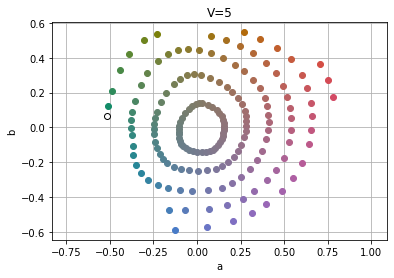
\includegraphics[width=\linewidth]{Grafiken/Vergleich_Munsell/oklab_munsell.png}
    \caption{Oklab}
    \label{fig:munsell_oklab}
  \end{subfigure}
  \begin{subfigure}[b]{0.3\linewidth}
    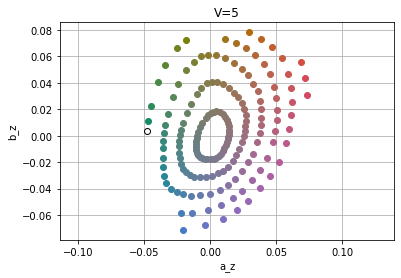
\includegraphics[width=\linewidth]{Grafiken/Vergleich_Munsell/jzazbz_munsell.png}
    \caption{JzAzBz}
    \label{fig:munsell_jzazbz}
  \end{subfigure}
  \begin{subfigure}[b]{0.3\linewidth}
    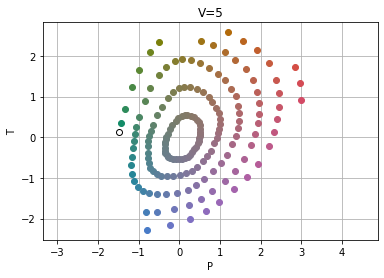
\includegraphics[width=\linewidth]{Grafiken/Vergleich_Munsell/ipt_munsell.png}
    \caption{IPT}
    \label{fig:munsell_ipt}
  \end{subfigure}
  
  \begin{subfigure}[b]{0.3\linewidth}
    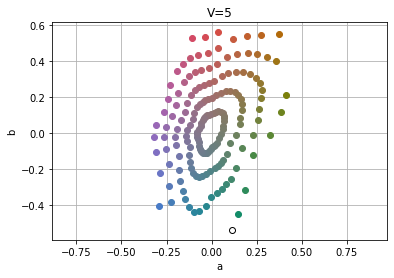
\includegraphics[width=\linewidth]{Grafiken/Vergleich_Munsell/hsv_munsell.png}
    \caption{HSV}
    \label{fig:munsell_hsv}
  \end{subfigure}
  \begin{subfigure}[b]{0.3\linewidth}
    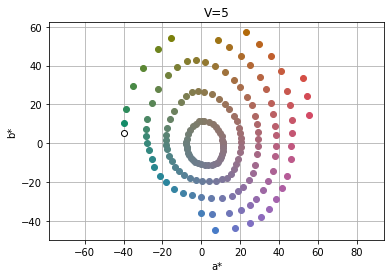
\includegraphics[width=\linewidth]{Grafiken/Vergleich_Munsell/cielab_munsell.png}
    \caption{CIELAB}
    \label{fig:munsell_cielab}
  \end{subfigure}
  \begin{subfigure}[b]{0.3\linewidth}
    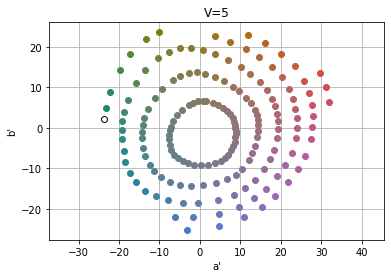
\includegraphics[width=\linewidth]{Grafiken/Vergleich_Munsell/cam16_munsell.png}
    \caption{CAM16-UCS}
    \label{fig:munsell_cam}
  \end{subfigure}
  
  \caption{Protts der Munsell Farben in den einzelnen Farbräumen. Quelle: ~\cite{Oklab_2020}}
  \label{fig:munsell_plots}
\end{figure}

\paragraph{Vergleich Farbverläufe}
Um nun nochmal auf das einleitende Problem mit den Farbverläufen zurückzukommen, 
werden in Grafik \ref{fig:blend_comp} nochmal ein Vergleich mit einem weiß-blauen Farbverlauf dargestellt.
Die Farbverläufe wurden mit denselben Farbräumen generiert, wie bei den Munsell Daten Plotts.
Auch bei diesen Farbverläufen sind einige Probleme zu erkennen, 
welche bereits bei dem Vergleich zwischen sRGB, perceptual und linear zu sehen waren.
Bei den Farbverläufen mit CIELAB und HSV ist eine deutliche Verschiebung des Hues hin zu Lila zu erkennen (Grafik \ref{fig:blend_hsv} und \ref{fig:blend_cielab}) und 
bei CAM16 scheinen die Farben zu schnell zu entsättigen, was den Übergang weniger gleichmäßig erscheinen lässt (Grafik \ref{fig:blend_cam}). 
Die übrigen drei Farbräume scheinen einen guten Farbverlauf zu liefern. 

\begin{figure}
  \centering
  \begin{subfigure}[b]{0.3\linewidth}
    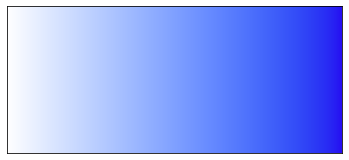
\includegraphics[width=\linewidth]{Grafiken/Vergleich_Farbverlauf/oklab_blend.png}
    \caption{Oklab}
    \label{fig:blend_oklab}
  \end{subfigure}
  \begin{subfigure}[b]{0.3\linewidth}
    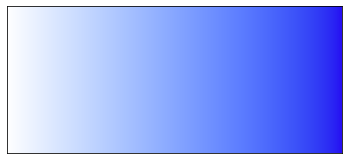
\includegraphics[width=\linewidth]{Grafiken/Vergleich_Farbverlauf/jzazbz_blend.png}
    \caption{JzAzBz}
    \label{fig:blend_jzazbz}
  \end{subfigure}
  \begin{subfigure}[b]{0.3\linewidth}
    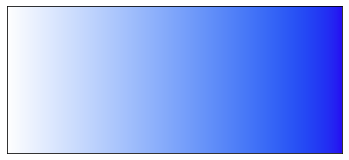
\includegraphics[width=\linewidth]{Grafiken/Vergleich_Farbverlauf/ipt_blend.png}
    \caption{IPT}
    \label{fig:blend_ipt}
  \end{subfigure}
  
  \begin{subfigure}[b]{0.3\linewidth}
    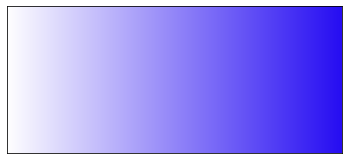
\includegraphics[width=\linewidth]{Grafiken/Vergleich_Farbverlauf/hsv_blend.png}
    \caption{HSV}
    \label{fig:blend_hsv}
  \end{subfigure}
  \begin{subfigure}[b]{0.3\linewidth}
    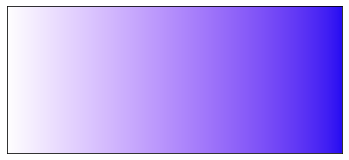
\includegraphics[width=\linewidth]{Grafiken/Vergleich_Farbverlauf/cielab_blend.png}
    \caption{CIELAB}
    \label{fig:blend_cielab}
  \end{subfigure}
  \begin{subfigure}[b]{0.3\linewidth}
    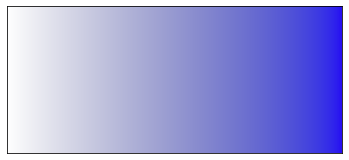
\includegraphics[width=\linewidth]{Grafiken/Vergleich_Farbverlauf/cam16_blend.png}
    \caption{CAM16-UCS}
    \label{fig:blend_cam}
  \end{subfigure}

  \caption{Blau-weiß Farbveräufe in den unterschiedlichen Farbräumen. Quelle: ~\cite{Oklab_2020}}
  \label{fig:blend_comp}
\end{figure}

\paragraph{Fazit}
Bei den Vergleichen ist zu erkennen, dass Oklab eine gute Alternative zu den anderen Farbräumen ist.
Oklab ist in der Lage, die wahrgenommene Helligkeit, das Chroma und den Farbton gut vorherzusagen, 
während es numerisch einfach und leicht zu übernehmen ist ~\cite{Oklab_2020}.
Besonders gut lassen sich die Vorteile von Oklab erkennen, 
wenn man einen Farbgradienten mit variierendem Hue, aber konstanter Helligkeit und Chroma erstellt. 
In Grafik \ref{fig:oklab_hsv} ist ein solcher Farbverlauf dargestellt, der gerade im Vergleich mit HSV eine deutliche konstantere Helligkeit zeigt. 
Zudem ist Oklab in der Lage wie in Gefik \ref{fig:hsv_lightness} zu erkennen, die gefühlten Helligkeitsunterschiede bei dem HSV Farbverlauf vorherzusagen.

\begin{figure}
  \centering
  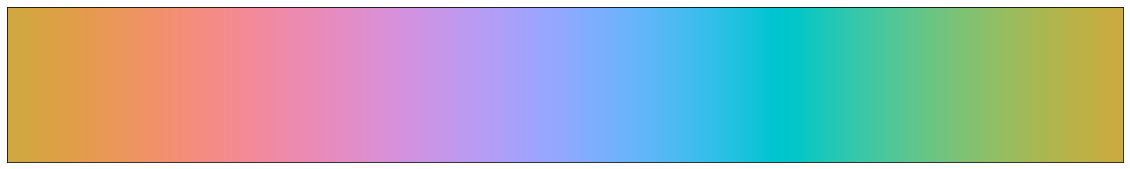
\includegraphics[width=0.5\linewidth]{Grafiken/Oklab_HSV/hue_oklab.png}
  \caption{Farbgradient mit konstanter Helligkeit und Chroma, aber variierendem Hue in Oklab}
  \label{fig:hue_oklab}
  
  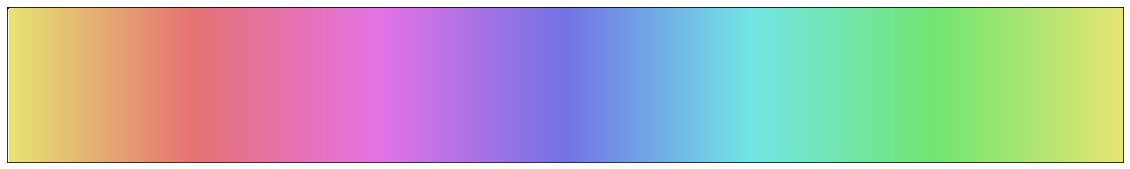
\includegraphics[width=0.5\linewidth]{Grafiken/Oklab_HSV/hue_hsv.png}
  \caption{Farbgradient mit konstanter Helligkeit und Chroma, aber variierendem Hue in HSV}
  \label{fig:hue_hsv}
  
  
\includegraphics[width=0.5\linewidth]{Grafiken/Oklab_HSV/hue_hsv_lightness.png}
  \caption{Wahrgenommene Helligkeit des HSV Farbverlaufs bestimmt durch Oklab}
  \label{fig:hsv_lightness}
  
  \caption{Vergleich von Farbgradienten mit Oklab und HSV Quelle: ~\cite{Oklab_2020}}
  \label{fig:oklab_hsv}
\end{figure}

\subsection{Oklab in der Praxis}
%anwendungsbeispiele und implementierungen

\newpage
% Bibliography
\printbibliography

\end{document}
